\subsubsection*{Difficulties}

The paper \cite{Riegler2016} only mentioned the application of a rule-base PART classifier on the dataset, further information was not provided.

\subsubsection*{Strategies}

In order to recreate the metrics we turned to the dataset paper \cite{Wang2016} for more details. The authors used the WEKA machine learning library\footnotetext{https://www.cs.waikato.ac.nz/ml/weka/ (accessed: 30.01.2020)} to calculate the weighted average of precision, recall and F1-score. \newline
However, we did not know which version of WEKA the authors used, so we downloaded the latest version (WEKA 3.8.4). \newline
We actually performed this task after the rebuilding of table \ref{table2} and used the preprocessed data from this approach (e.g. we used the visual data where we kept only the first row). Reading the files into WEKA was rather straightforward but the test options for the rule-based PART classifier were not declared in one of the papers either. So we decided to use the test sets of the features and let WEKA compute the scores. A resulting model is shown in figure \ref{weka}.

\begin{figure}[h]
	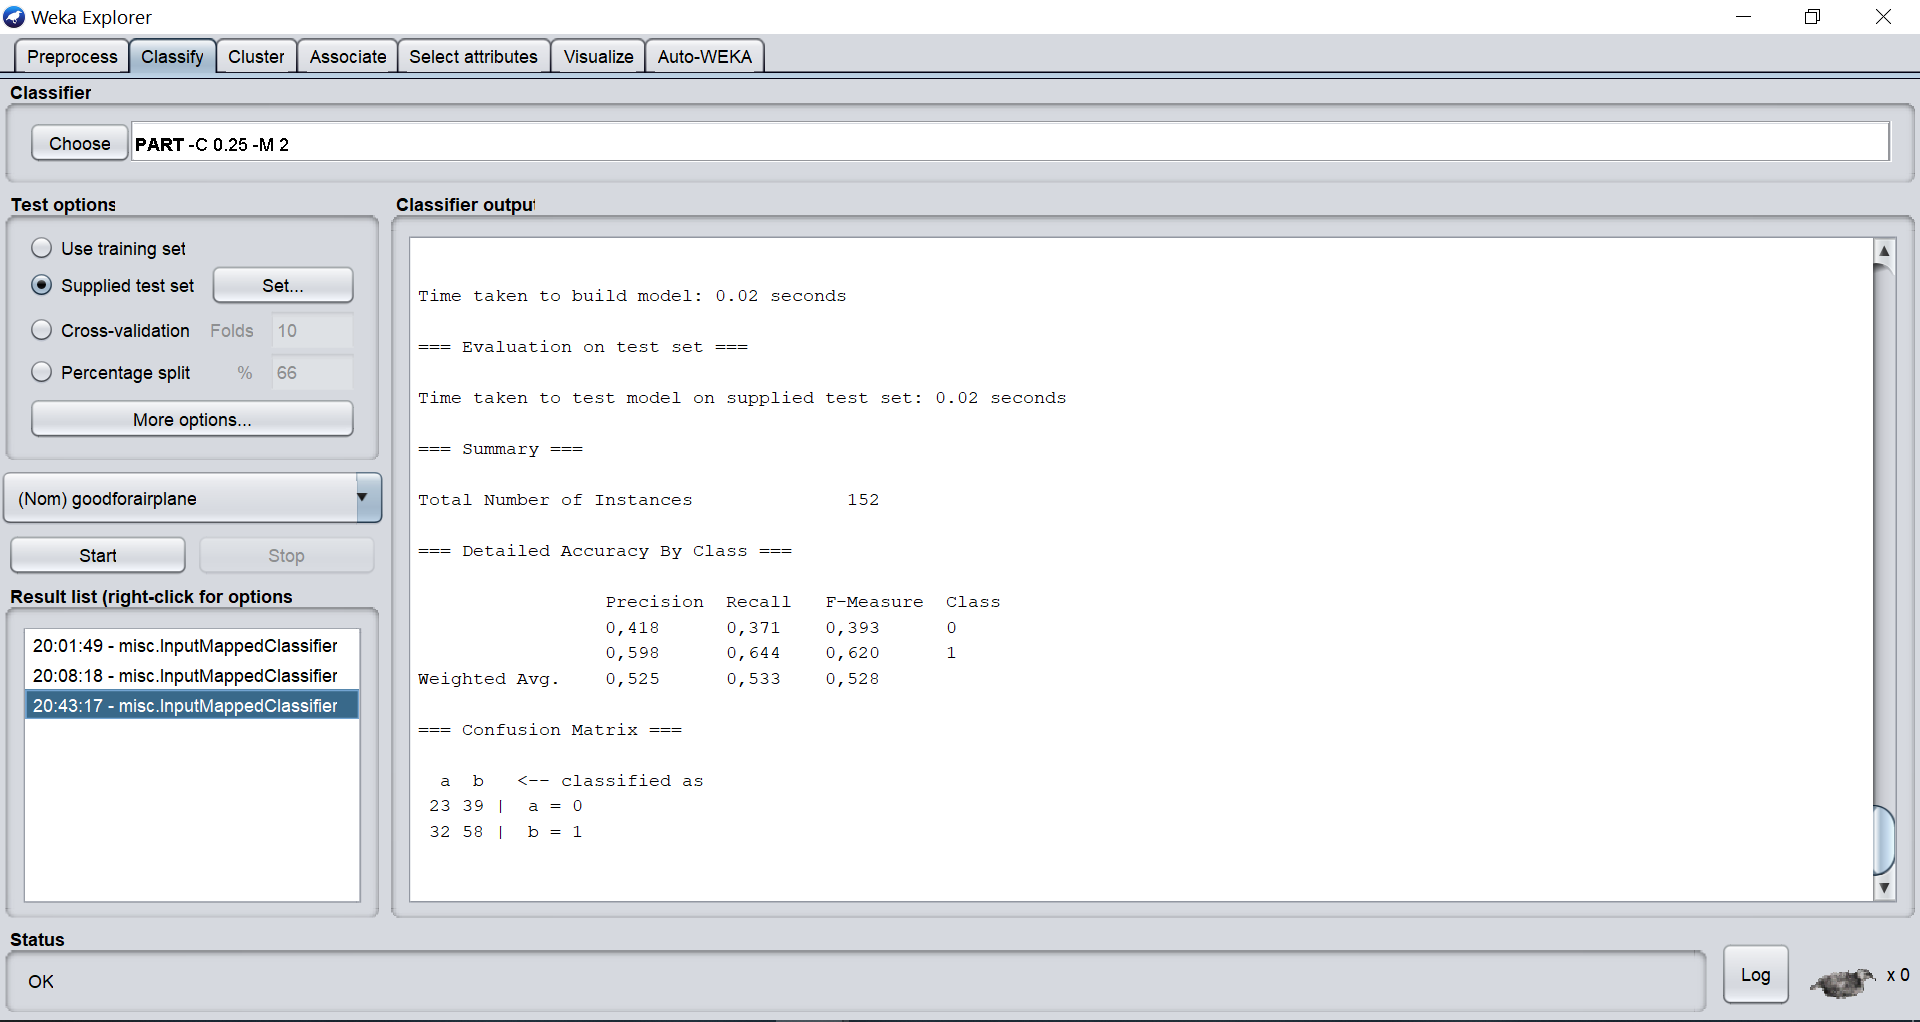
\includegraphics[width=0.45\textwidth]{weka.png}
	\caption{Screenshot of the resulting model for the metadata after applying the rule-base PART classifier}
	\label{weka}
\end{figure}


\subsubsection*{Key Findings}

It is not sufficient to state which classifier was applied, but also which software (-version) was used and which preprocessing steps were performed. WEKA gives the user a variety of options which makes it quite important to recite the performed steps to assure reproducability. \newline
Nevertheless, we obtained satsifying results that were comparable to the ones in the papers.

